\documentclass[12pt,a4paper]{article}
\usepackage{fullpage}
\usepackage[top=2cm, bottom=4.5cm, left=2.5cm, right=2.5cm]{geometry}
\usepackage{amsmath,amsthm,amsfonts,amssymb,amscd}
\usepackage{lastpage}
\usepackage{enumerate}
\usepackage{fancyhdr}
\usepackage{mathrsfs}
\usepackage{xcolor}
\usepackage{graphicx}
\usepackage{listings}
\usepackage{hyperref}
\usepackage{txfonts}
\usepackage{titlesec}
\usepackage{floatflt}
\usepackage{wrapfig}

\hypersetup{%
  colorlinks=true,
  linkcolor=blue,
  linkbordercolor={0 0 1}
}


\newcommand\course{8.03x - Vibrations and Waves}
\newcommand\hwnumber{1}               
\newcommand\MyName{Syed Suhaib Ahmad}
 
\renewcommand\lstlistingname{Algorithm}
\renewcommand\lstlistlistingname{Algorithms}
\def\lstlistingautorefname{Alg.}

\setlength{\parindent}{0.0in}
\setlength{\parskip}{0.05in}



\pagestyle{fancyplain}
\headheight 35pt
\lhead{\course}
\chead{\large\textbf{Problem Set 3}}
\rhead{\MyName{}}
\lfoot{}
\cfoot{\small\thepage}
\rfoot{}
\headsep 1.5em

\begin{document}

\subsubsection*{Problem 3.1 - Coupled oscillators using two springs}
\begin{floatingfigure}[r]{0.2\textwidth}
\vspace{-0.8em} % Adjust this value to align with the paragraph
\centering
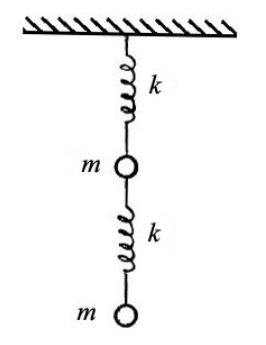
\includegraphics[width=0.17\textwidth]{figs/fig_prob_3.1.png}
\end{floatingfigure}
Two equal masses are connected as shown with two identical massless
springs of spring constant $k$. Considering only motion in the vertical direction, show that the angular frequencies of the two normal modes are given by $\omega^2=(3\pm\sqrt{5})k/2m$ and hence that the ratio of the normal mode frequencies is $(\sqrt{5}+1)/(\sqrt{5}-1)$. Find the ratio of amplitudes of the two masses in each separate mode. (\textit{Note:} You need not consider the gravitational forces acting on the masses, because they are independent of the displacements and hence do not contribute to the restoring forces that cause the oscillations. The gravitational forces merely cause a shift in the equilibrium positions of the masses, and you do not have to find what those shifts are.)
\newline
\\
\textbf{Solution}
\\
\\Assuming downwards the positive direction, let there is an extension $x_1$ in the top spring and an extension $x_2$ in bottom spring $(x_2>x_1)$. Due to these displacements, there are restoring forces on both masses, $F_{\text{res1}}$ and $F_{\text{res2}}$.
\[F_{\text{res1}}=k(x_2-x_1)-kx_1\,\,\,\,\,\,\,\,\,\,\text{(upper mass)}\]
\[F_{\text{res2}}=-k(x_2-x_1)\,\,\,\,\,\,\,\,\,\,\text{(lower mass)}\]
Since these are the only forces responsible for motion of masses (to avoid confusion, let $m_1$ be the upper mass and $m_2$ be the lower mass), we have the following coupled differential equations from Newton's second law
\begin{equation}
    m_1\frac{d^2x_1}{dt^2}=k(x_2-x_1)-kx_1\Rightarrow\frac{d^2x_1}{dt^2}+\omega_s^2(2x_1-x_2)=0
\end{equation}
\begin{equation}
    m_2\frac{d^2x_2}{dt^2}=-k(x_2-x_1)\Rightarrow\frac{d^2x_2}{dt^2}+\omega_s^2(x_2-x_1)=0,
\end{equation}
where $\omega_s^2=k/m$. Both Eq. (1) and Eq. (2) are similar to a differential equation involving simple harmonic oscillation. Thus, we can “guess” that solutions to both equations are of the form
\[x_1(t)=A_1\cos\omega t\,\,\,\,\,\text{and}\,\,\,\,\,x_2(t)=A_2\cos\omega t.\]
Taking second derivatives of $x_1(t)$ and $x_2(t)$ and then substituting them into Eq. (1) and Eq. (2):
\[\,\,\,(1)\,\,\,\,\,-A_1\omega^2\cos\omega t+\omega_s^2\cos\omega t(2A_1-A_2)=0\]
\begin{equation}
    -A_1\omega^2+2A_1\omega_s^2-A_2\omega_s^2=0\Rightarrow \frac{A_1}{A_2}=\frac{\omega_s^2}{2\omega_s^2-\omega^2}
\end{equation}
\[(2)\,\,\,\,\,-A_2\omega^2\cos\omega t+\omega_s^2\cos\omega t(A_2-A_1)=0\]
\begin{equation}
    -A_2\omega^2+A_2\omega_s^2-A_1\omega_s^2=0\Rightarrow \frac{A_1}{A_2}=\frac{\omega_s^2-\omega^2}{\omega_s^2}.
\end{equation}
Hence, now we have
\[\frac{\omega_s^2}{2\omega_s^2-\omega^2}=\frac{\omega_s^2-\omega^2}{\omega_s^2}\]
\[\omega_s^4=\left(2\omega_s^2-\omega^2\right)\left(\omega_s^2-\omega^2\right)\]
\[\omega_s^4=2\omega_s^4-2\omega^2\omega_s^2-\omega^2\omega_s^2+\omega^4\]
\[\omega^4-3\omega^2\omega_s^2+\omega_s^4=0\]
Solving for $\omega_2$:
\[\omega^2=\frac{3\omega_s^2\pm\sqrt{9\omega_s^4-4\omega_s^4}}{2}=\frac{\omega_s^2}{2}\left(3\pm\sqrt{5}\right)=\frac{k}{2m}\left(3\pm\sqrt{5}\right).\]
Therefore, the two normal mode frequencies are
\begin{equation}
    \omega_-=\sqrt{\frac{k}{2m}\left(3-\sqrt{5}\right)},\,\,\,\,\,\,\,\,\,\,\omega_+=\sqrt{\frac{k}{2m}\left(3+\sqrt{5}\right)}
\end{equation}
and their ratio is
\[\frac{\omega_+}{\omega_-}=\sqrt{\frac{3+\sqrt{5}}{3-\sqrt{5}}}=\frac{\sqrt{5}+1}{\sqrt{5}-1}.\]
For $\omega_-$, the ratio of amplitudes is given by
\[\frac{A_1}{A_2}=\frac{\omega_s^2-\omega^2}{\omega_s^2}=\frac{k/m-(k/2m)\left(3-\sqrt{5}\right)}{k/m}=\frac{\sqrt{5}-1}{2}\]
and for $\omega_+$,
\[\frac{A_1}{A_2}=\frac{k/m-(k/2m)\left(3+\sqrt{5}\right)}{k/m}=\frac{-\sqrt{5}-1}{2}.\]
\\
\subsubsection*{Problem 3.2 - Coupled spring and pendulum}
The sketch shows a mass $M_1$ on a frictionless plane connected to support $O$ by a spring of stiffness $k$. Mass $M_2$ is supported by a string of length $l$ from $M_1$. $OA$ is the length of the relaxed spring. $x_1$ and $x_2$ are the positions of $M_1$ and $M_2$, respectively, relative to point $A$. The figure is not to scale; $x_1$ is much smaller than $OA$.
\begin{enumerate}
    \item[(a)]Write down the differential equations of motion for each mass.
    \item[(b)]For $M_1=M_2=M$, calculate the normal mode frequencies (use the small angle approximation for the pendulum).
    \item[(c)]What are the associated ratios of the amplitude of the two masses?
    \begin{figure}[h]
        \centering
        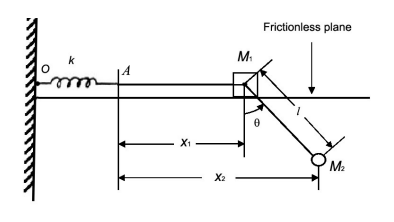
\includegraphics[width=0.6\linewidth]{figs/fig_prob_3.2.png}
        %\caption{Caption}
       % \label{fig:enter-label}
    \end{figure}
\end{enumerate}
\textbf{Solution(a)}
\\
\\For a displacement $x_1$ in the spring, the restoring force on $M_1$ is $-kx$. Moreover, since the string is connected to $M_1$, the horizontal component also acts on it. Therefore, differential equation of motion for $M_1$ is
\begin{equation}
    M_1\frac{d^2x_1}{dt^2}=-kx_1+T\sin\theta.
\end{equation}
Given that the vertical component of tension is equal to the weight of $M_2$.
\[T\cos\theta=M_2g.\]
Using the small angle approximation, we find that $T\approx M_2g$. From the given figure, $\sin\theta=(x_2-x_1)/l$. As mentioned in previous problem, $k/M_1=\omega_s^2$. Also, $g/l=\omega_p^2$, the natural frequency of the pendulum. We substitute these values into Eq. (6) to obtain
\[M_1\frac{d^2x_1}{dt^2}=-kx_1+\frac{M_2g}{l}(x_2-x_1)\]
\begin{equation}
    \frac{d^2x_1}{dt^2}+\omega_s^2x_1-\omega_p^2\frac{M_2}{M_1}(x_2-x_1)=0.
\end{equation}
As far as $M_2$ is concerned, only the horizontal component of tension acts on it in the $x-$direction.
\[M_2\frac{d^2x_2}{dt^2}=-T\sin\theta\]
\[M_2\frac{d^2x_2}{dt^2}=-\frac{M_2g}{l}(x_2-x_1)\]
\begin{equation}
    \frac{d^2x_2}{dt^2}+\omega_p^2(x_2-x_1)=0.
\end{equation}
\textbf{Solution(b)}
\\
\\For $M_1=M_2=M$, we have the following coupled differential equations
\begin{equation}
   \frac{d^2x_1}{dt^2}+\left(\omega_s^2+\omega_p^2\right)x_1-\omega_p^2x_2=0 
\end{equation}
\begin{equation}
    \frac{d^2x_2}{dt^2}+\omega_p^2(x_2-x_1)=0.
\end{equation}
\newpage
Let $x_1=A_1\cos\omega t$ and $x_2=A_2\cos\omega t$. Then, $d^2x_1/dt^2=-A_1\omega^2\cos\omega t$ and $d^2x_2/dt^2=-A_2\omega^2\cos\omega t$. Putting $d^2x_1/dt^2$, $x_1$ and $x_2$ into Eq. (9)
\begin{equation}
    -A_1\omega^2+A_1(\omega_s^2+\omega_p^2)-A_2\omega_p^2=0
\end{equation}
and then similarly; $d^2x_2/dt^2$, $x_1$ and $x_2$ into Eq. (10)
\begin{equation}
    -A_2\omega^2+(A_2-A_1)\omega_p^2=0.
\end{equation}
We can combine equations (11) and (12) to write them in the form of a single matrix equation.
\begin{equation}
    \begin{pmatrix}
    \omega_s^2+\omega_p^2-\omega^2 & -\omega_p^2\\
    -\omega_p^2 & \omega_p^2-\omega^2
\end{pmatrix}
\begin{pmatrix}
    A_1\\
    A_2
\end{pmatrix}=
\begin{pmatrix}
    0\\
    0
\end{pmatrix}
\end{equation}
For non-trivial solutions ($A_1$ and $A_2$ $\neq0$), the coefficient matrix must be singular.
\[\begin{vmatrix}
    \omega_s^2+\omega_p^2-\omega^2 & -\omega_p^2\\
    -\omega_p^2 & \omega_p^2-\omega^2
\end{vmatrix}=0\]
\[\omega_p^4-\left(\omega_s^2+\omega_p^2-\omega^2\right)\left(\omega_p^2-\omega^2\right)=0\]
\[\omega_p^4=\omega_s^2\omega_p^2-\omega_s^2\omega^2+\omega_p^4-\omega_p^2\omega^2-\omega_p^2\omega^2+\omega^4\]
\[\omega^4-\omega^2\left(2\omega_p^2+\omega_s^2\right)+\omega_s^2\omega_p^2=0\]
\[\omega^2=\frac{2\omega_p^2+\omega_s^2\pm\sqrt{\left(2\omega_p^2+\omega_s^2\right)^2-4\omega_s^2\omega_p^2}}{2}\]
\[\omega=\left(\frac{2\omega_p^2+\omega_s^2}{2}\pm\frac{\sqrt{4\omega_p^4+\omega_s^4}}{2}\right)^{1/2}\]
Finally, the normal mode frequencies are
\begin{equation}
    \omega_-\left(\frac{2\omega_p^2+\omega_s^2}{2}-\frac{\sqrt{4\omega_p^4+\omega_s^4}}{2}\right)^{1/2}\,\,\,\,\,\text{and}\,\,\,\,\,\omega_+=\left(\frac{2\omega_p^2+\omega_s^2}{2}+\frac{\sqrt{4\omega_p^4+\omega_s^4}}{2}\right)^{1/2}.
\end{equation}
\textbf{Solution(c)}
\\
\\We can manipulate either of the equations (11) or (12) to find the ratio of amplitudes.
\begin{equation}
    \frac{A_1}{A_2}=\frac{\omega_p^2}{\omega_s^2+\omega_p^2-\omega^2}.
\end{equation}
Substituting $\omega_-$ and $\omega_+$ into Eq. (15) separately, gives the ratio of amplitudes at each frequency. 
\[\left(\frac{A_1}{A_2}\right)_-=\frac{2\omega_p^2}{\omega_s^2+\sqrt{4\omega_p^4+\omega_s^4}}\,\,\,\,\,\text{and}\,\,\,\,\,\left(\frac{A_1}{A_2}\right)_+=\frac{2\omega_p^2}{\omega_s^2-\sqrt{4\omega_p^4+\omega_s^4}}.\]

\subsubsection*{Problem 3.3 - Coupled oscillators using three springs}
Two springs, each of constant $k$, support a rigid, massless platform to which a mass $m$ is firmly attached. The position of this mass is $y_1(t$). A second mass m hangs at the end of another spring (of constant $k$) from the center of the platform, as shown in the sketch. The position of this second mass is $y_2(t)$. Assume that the two longer springs move together with the same frequency and in the same plane.
\begin{figure}[h]
    \centering
    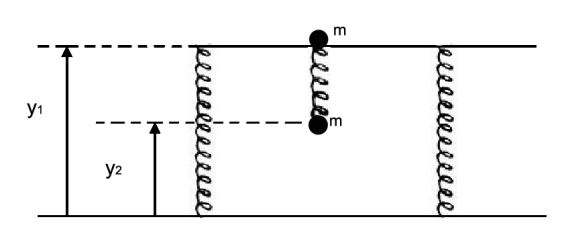
\includegraphics[width=0.6\linewidth]{figs/fig_prob_3.3.png}
    %\caption{Caption}
   % \label{fig:enter-label}
\end{figure}
\begin{enumerate}
    \item[(a)]Write the differential equations of motion for each of the masses.
    \item[(b)]Solve the equations to find the normal mode frequencies and find suitable expressions for $y_1(t)$ and $y_2(t)$.
    \item[(c)]Sketch the configuration of the system for each of the two normal modes. Label the sketches to indicate which configuration corresponds to the normal mode with low frequency $\omega_1$, and which configuration corresponds to the mode with high frequency $\omega_2$.
\end{enumerate}
\textbf{Solution(a)}
\\
\\Let the upper and lower masses are initially at a height of $h_1$ and $h_2$ respectively. If the platform is raised by a displacement $x_1$, upper mass would have a displacement of $x_1$ and the hanging mass would have a displacement of $x_2$. Both displacements are from the equilibrium positions of masses. Assuming $x_1>x_2$ and upwards is positive, we have the following differential equations for the two masses
\begin{equation}
    m\frac{d^2x_1}{dt^2}=-2kx_1-k(x_1-x_2)\Rightarrow\frac{d^2x_1}{dt^2}+3\omega_p^2x_1-\omega_p^2x_2=0.
\end{equation}
\begin{equation}
  m\frac{d^2x_2}{dt^2}=k(x_1-x_2)\Rightarrow\frac{d^2x_2}{dt^2}-\omega_p^2x_1+\omega_p^2x_2=0.
\end{equation}
\textbf{Solution(b)}
\\
\\If $x_1=A\cos\omega t$ and $x_2=B\cos\omega t$, then $d^2x_1/dt^2=-A\omega^2\cos\omega t$ and $d^2x_2/dt^2=-B\omega^2\cos\omega t$. Substituting $x_1$, $x_2$, $d^2x_1/dt^2$ and $d^2x_2/dt^2$ into equations (16) and (17) gives
\begin{equation}
    A\left(3\omega_p^2-\omega^2\right)-B\omega_p^2=0
\end{equation}
\begin{equation}
   -A\omega_p^2+B\left(\omega_p^2-\omega^2\right)=0
\end{equation}
Writing the above equations in the form of matrices:
\begin{equation}
    \begin{pmatrix}
        3\omega_p^2-\omega^2 & -\omega_p^2\\
        -\omega_p^2 & \omega_p^2-\omega^2
    \end{pmatrix}
    \begin{pmatrix}
        A\\
        B
    \end{pmatrix}=
    \begin{pmatrix}
        0\\
        0\\
    \end{pmatrix}
    .
\end{equation}
For non-trivial solutions,
\[\begin{vmatrix}
     3\omega_p^2-\omega^2 & -\omega_p^2\\
        -\omega_p^2 & \omega_p^2-\omega^2
\end{vmatrix}=0\]
\[\omega^4-4\omega^2\omega_p^2+2\omega_p^4=0\]
\[\omega^2=\omega_p^2\left(2\pm\sqrt{2}\right).\]
Now, we have
  \[\omega_-=\omega_p\left(2-\sqrt{2}\right)^{1/2},\,\,\,\,\,\,\,\,\,\,\omega_+=\omega_p\left(2+\sqrt{2}\right)^{1/2},\]
\begin{equation}
    \left(\frac{B}{A}\right)_-=1+\sqrt{2}\,\,\,\,\,\text{and}\,\,\,\,\,\left(\frac{B}{A}\right)_+=1-\sqrt{2}.
\end{equation}
If the amplitude of $x_1$ is $A_-$ in the first normal mode solution, then according to Eq. (21), $x_2$'s maximum value would be $\left(1+\sqrt{2}\right)A_-$. Similarly, for $\omega_+$, the amplitudes of $x_1$ and $x_2$ would be $A_+$ and $\left(1-\sqrt{2}\right)A_+$ respectively. Therefore, the normal mode solutions are
\begin{equation}
    \begin{pmatrix}
    x_1\\
    x_2
\end{pmatrix}_-=A_-\begin{pmatrix}
    \cos(\omega_-t)\\
    \left(1+\sqrt{2}\right)\cos(\omega_-t)
\end{pmatrix}\,\,\,\,\,\text{and}\,\,\,\,\,\begin{pmatrix}
    x_1\\
    x_2
\end{pmatrix}_+=A_+\begin{pmatrix}
    \cos(\omega_+t)\\
    \left(1-\sqrt{2}\right)\cos(\omega_+t)
\end{pmatrix}.
\end{equation}
The general solutions for $y_1$ and $y_2$ are a superposition of the normal mode solutions and the respective heights of the masses.
\begin{equation}
    \begin{pmatrix}
    y_1\\
    y_2
\end{pmatrix}=\begin{pmatrix}
    h_1\\
    h_2
\end{pmatrix}+A_-\begin{pmatrix}
    \cos(\omega_-t)\\
    \left(1+\sqrt{2}\right)\cos(\omega_-t)
\end{pmatrix}+A_+\begin{pmatrix}
    \cos(\omega_+t)\\
    \left(1-\sqrt{2}\right)\cos(\omega_+t)
\end{pmatrix}.
\end{equation}

\textbf{Solution(c)}
\begin{figure}[h]
    \centering
    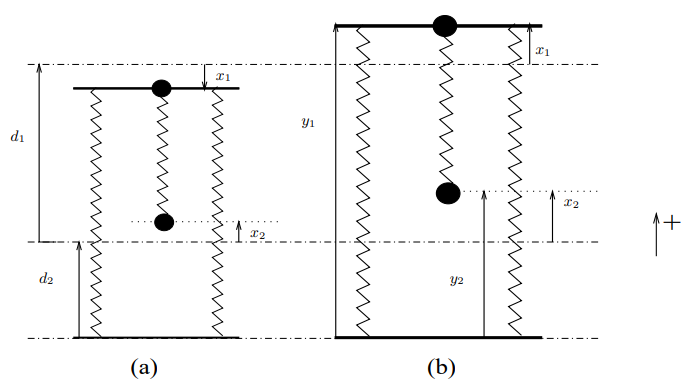
\includegraphics[width=0.8\linewidth]{figs/fig_sol_3.3c.png}
  %  \caption{Caption}
 %   \label{fig:enter-label}
\end{figure}
\\Figure (a) shows the configuration for the frequency $\omega_-$ and figure (b) for $\omega_+$. Both figures clearly show the specific properties of the normal mode solutions; at $\omega_+$, both oscillations are out of phase and at $\omega_-$, oscillations are in phase with bigger amplitudes.
\newpage
\subsubsection*{Problem 3.4 - Driven coupled oscillator}
Use the figure under problem 3.2 but now the left end of the spring is not attached. Instead, we oscillate it harmonically in horizontal direction. Its position $X(t)$ is given by $X_0\cos(\omega t)$.
\begin{enumerate}
    \item[(a)]Write down the differential equation of motion for each mass.
    \item[(b)]Let both masses be $M$. What now are the amplitudes (steady state) of the two masses as a function of $k$, $M$, $X_0$, $l$ and $\omega$? (\textit{Hint: Use Cramer’s rule!})
    \item[(c)]Make careful plots of the amplitude of the two masses as a function of $\omega$. Observe the phases. Be quantitative at $\omega=0$ and also indicate frequencies that are “special”.
    \item[(d)]There is one frequency for which one mass stands still and the other oscillates. What is that frequency? You should recognize this answer as “very familiar”. What’s going on here?
\end{enumerate}
\textbf{Solution(a)}
\\
\\With the introduction of this harmonic displacement $X(t)$, we only need to change Eq. (7) for $M_1$, that is, now the restoring force on $M_1$ is $-k(x_1-X_0\cos\omega t)$. However, the equation of motion for $M_2$ remains the same as Eq.(8). Thus, the differential equation for $M_1$ is
\[\frac{d^2x_1}{dt^2}+\omega_s^2(x_1-X_0\cos\omega t)-\omega_p^2\frac{M_2}{M_1}(x_2-x_1)=0\]
\begin{equation}
    \frac{d^2x_1}{dt^2}+\omega_s^2x_1-\omega_p^2\frac{M_2}{M_1}(x_2-x_1)=\omega_s^2X_0\cos\omega t.
\end{equation}
For $M_2$:
\begin{equation}
     \frac{d^2x_2}{dt^2}+\omega_p^2(x_2-x_1)=0.
\end{equation}
\textbf{Solution(b)}
\\
\\Letting $x_1=C_1\cos\omega t$ and $x_2=C_2\cos\omega t$, and then substituting $x_1$, $x_2$ and their second derivatives into equations (24) and (25) gives the two following equations:
\begin{equation}
    C_1\left(-\omega^2+\omega_s^2+\omega_p^2\right)-C_2\omega_p^2=\omega_s^2X_0
\end{equation}
\begin{equation}
    -C_1\omega_p^2+C_2\left(\omega_p^2-\omega^2\right)=0.
\end{equation}
This system of two linear equations can be written as a matrix equation in the following way
\begin{equation}
    \begin{pmatrix}
        -\omega^2+\omega_s^2+\omega_p^2 & -\omega_p^2 \\
        -\omega_p^2 & \omega_p^2-\omega^2
    \end{pmatrix}
    \begin{pmatrix}
        C_1 \\
        C_2
    \end{pmatrix}=
    \begin{pmatrix}
        \omega_s^2X_0 \\
        0
    \end{pmatrix}.
\end{equation}
Using Cramer's rule, we have
\begin{equation}
    C_1=\frac{\begin{vmatrix}
         \omega_s^2X_0 & -\omega_p^2 \\
        0 & \omega_p^2-\omega^2
    \end{vmatrix}}{\begin{vmatrix}
        -\omega^2+\omega_s^2+\omega_p^2 & -\omega_p^2 \\
        -\omega_p^2 & \omega_p^2-\omega^2
    \end{vmatrix}}=\frac{kX_0\left(g-l\omega^2\right)}{kg+Ml\omega^4-(kl+2Mg)\omega^2}
\end{equation}

and
\begin{equation}
    C_2=\frac{\begin{vmatrix}
       -\omega^2+\omega_s^2+\omega_p^2  & \omega_s^2X_0 \\
        -\omega_p^2 & 0
    \end{vmatrix}}{\begin{vmatrix}
        -\omega^2+\omega_s^2+\omega_p^2 & -\omega_p^2 \\
        -\omega_p^2 & \omega_p^2-\omega^2
    \end{vmatrix}}=\frac{kgX_0}{kg+Ml\omega^4-(kl+2Mg)\omega^2}\,.
\end{equation}
\textbf{Solution(c)}
\begin{figure}[h]
    \centering
    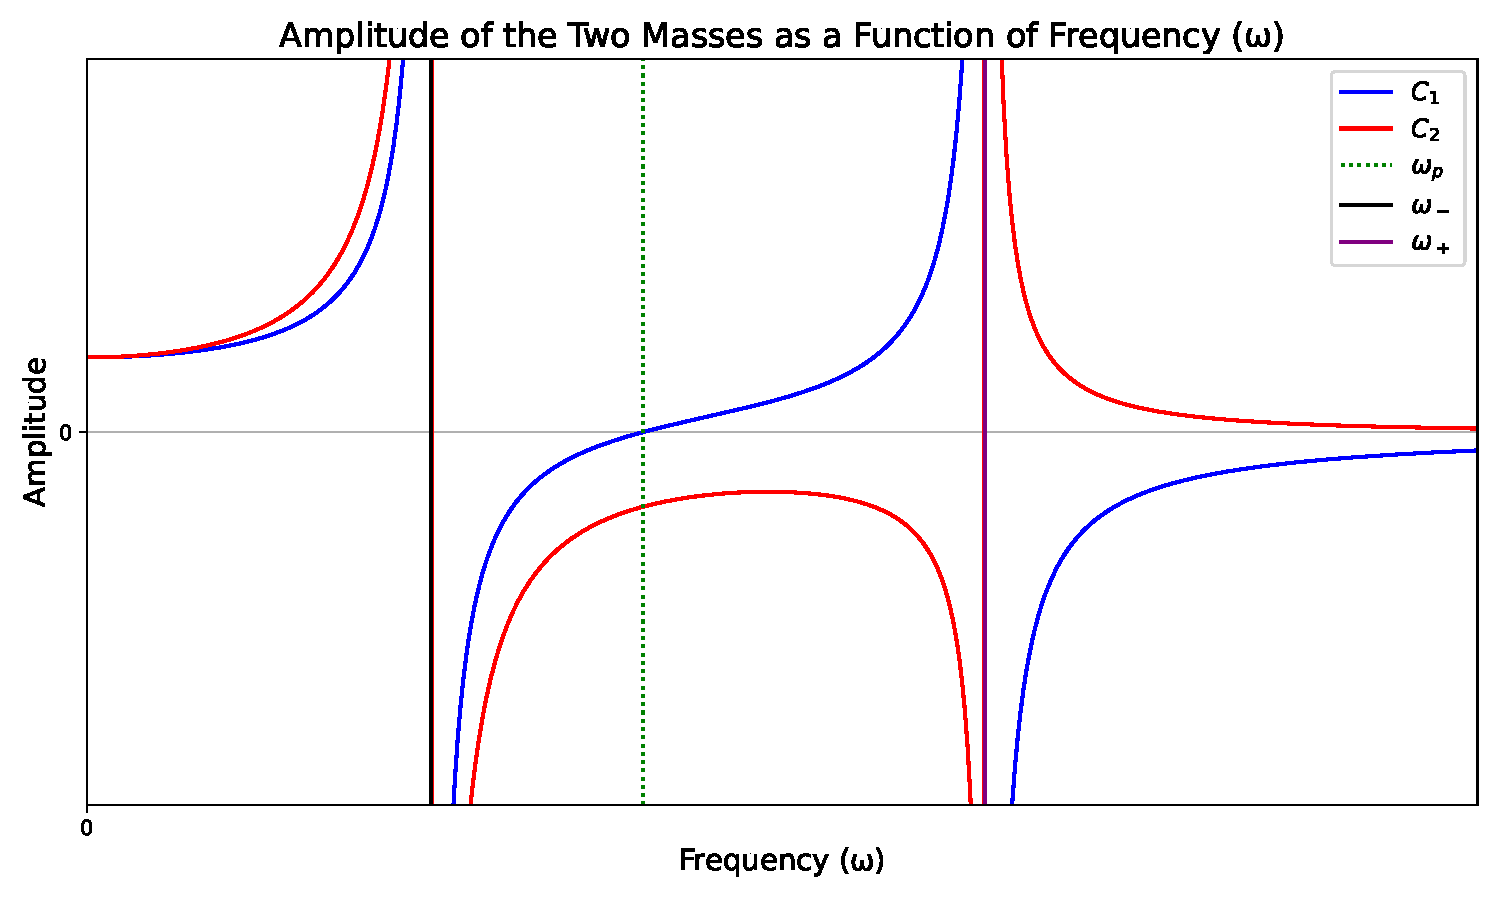
\includegraphics[width=1\linewidth]{figs/fig_sol_3.4c.pdf}
   % \caption{Caption}
  %  \label{fig:enter-label}
\end{figure}
\\At $\omega=0$, $C_1=C_2=X_0$, meaning there is no oscillation and the displacement of pendulum and spring is merely because of the driven harmonic displacement. Moreover, the special frequencies are $\omega_-$ and $\omega_+$. At $\omega=\omega_-$ or near it, both amplitudes are in phase and vice versa. $C_1=0$ at $\omega=\omega_p$, the natural frequency of pendulum, this means only the spring oscillates at this point and spring remains at rest.
\\
\\\textbf{Solution(d)}
\\
\\As mentioned in part (c), at $\omega=\omega_p$; only the pendulum oscillates and spring stays still. We can easily see that $C_2$, never becomes zero unless $\omega\rightarrow\infty$. However, $C_1$ is zero when $\omega^2=g/l$.\\
\\
It is important to note that this exact state is impossible to achieve in real world due to damping. For instance, when spring is not oscillating, the vectorial sum of spring force and horizontal component of tension on $M_1$ is zero. However, when spring is at rest, there no driving force on pendulum and in the presence of damping, its amplitude will start to decrease. Consequently, the tension will decrease in $x-$direction (as pendulum slows down) meaning the net horizontal forces on spring mass are not zero anymore, thus $M_1$ will start to move again. In conclusion, this state of the system is extremely unstable in real world.


\end{document}